\chapter{THÔNG TIN SAI LỆCH VÀ CƠ CHẾ LAN TRUYỀN THÔNG TIN SAI LỆCH}
\label{chap:2}
Chương 1 đã trình bày tổng quan về các tác hại mà thông tin sai lệch gây ra đối với người dùng MXH. Những hậu quả to lớn của thông tin sai lệch trên MXH có thể thấy rõ trên hai khía cạnh sau: 

- Về tâm lý, chính trị: Những thông tin sai lệch ảnh hưởng tiêu cực đến tâm lý, đời sống tinh thần của người dùng khi chúng được phát tán trên mạng. Nó có thể ảnh hưởng đến tinh thần, thái độ, thậm chí cả chính trị của khu vực người dùng sinh sống. 

- Về kinh tế, những thông tin sai lệnh tiêu cực về sản phẩm của một doanh nghiêp ảnh hưởng xấu đến tài chính, giá bán, doanh thu, và thậm chí là thương hiệu của doanh nghiệp đó. 

Những tác hại kể trên cho thấy việc đối phó với các thông tin sai lệch là vô cùng cấp bách. Việc phát hiện ngồn thông tin sai lệch là cơ sở cho các giải pháp ngăn chặn sự phát tán của chúng. Nguồn phát tán thông tin sai lệch có thể được phát hiện thông qua khảo sát người dùng hoặc các phương pháp khai phá dữ liệu.

Để có thể đưa ra giải pháp hiệu quả trong việc ngăn chặn sự lan truyền của thông tin sai lệch, trước tiên chúng ta phải hiểu được cơ chế thông tin sai lệch lan truyền trên MXH. Chương này phân tích quá trình lan truyền thông tin sai lệch dưới hai mô hình lan truyền: Mô hình bậc độc lập và mô hình ngưỡng tuyến tính, đây là hai mô hình phổ biến, được sử dụng rộng rãi trong các công trình nghiên cứu liên quan đến vấn đề lan truyền thông tin, lan truyền ảnh hưởng trên MXH.


\section{Mô hình lan truyền thông tin}
Thông tin được phát tán trên các MXH từ người dùng này đến người dùng khác thông qua nhiều hoạt động đăng bài, chia sẻ, bình luận. Kempe \cite{kemple1} là người đầu tiên đưa ra các mô hình phát tán thông tin, trong đó đã đưa ra hai mô hình phát tán thông tin cơ bản là Mô hình tầng độc lập (Independent Cascade – IC) và Mô hình ngưỡng tuyến tính (Linear Threshold – LT). Hai mô hình này sau đó đã được sử dụng rộng rãi trong các bài toán liên quan đến lan truyền, phát tán thông tin.

Các mô hình phát tán thông tin là cơ sở cho việc nghiên cứu hạn chế thông tin sai lệch cũng như các tin đồn thất thiệt. Các nghiên cứu về chủ đề này những năm gần đây đều dựa trên hai mô hình IC, LT và các biến thể của chúng \cite{kemple2}, \cite{Golden}, \cite{Carnes}. Theo đó, một mạng xã hội được biểu diễn bởi các thành phần như sau:
\begin {itemize}
	\item V là tập hợp các đỉnh của đồ thị, |V| = n, biểu diễn những người dùng tồn tại trong MXH.

	\item E $\subset$ VxV hợp các cạnh của đồ thị, |E| = m gồm m cạnh có hướng, biểu diễn mối quan hệ giữa các cá nhân trong MXH.

	\item w(u,v) là trọng số của cạnh (u, v) là một số thực dương biểu diễn cho các tần số tương tác, trao đổi giữa hai người dùng. w(u, v) = 0 nếu giữa hai đỉnh u và v không tồn tại cạnh, w(u, v) > 0 nếu giữa u và v tồn tại cạnh nối.
\end {itemize}
Do G là đồ thị có hướng nên cạnh (u,v) được gọi là cạnh đi ra từ u, cạnh (v,u) được gọi là cạnh đi vào đỉnh u. Ta ký hiệu N$_{out}$(u) và N$_{in}$(u) tương ứng là tập hợp các đỉnh hàng xóm đi ra và đi vào đỉnh u.

Quá trình lan truyền thông tin theo các bước thời gian rời rạc, với thời gian t = 0, 1, 2, ... Gọi S$_{t}$ $\subset$ V là tập các đỉnh ở trạng thái {\itshape kích hoạt} tại thời điểm t. Tập các đỉnh là nguồn phát tán thông tin sai lệch ban đầu hay còn gọi là tập hạt giống, kí hiệu là S$_{0}$

Tại mỗi bước thời gian t, đỉnh u ở trạng thái kích hoạt nếu u $\subset$ S$_{0}$ hoặc u nhận được thông tin sai lệch từ các đỉnh hàng xóm ở trạng thái kích hoạt và chấp nhận thông tin này để tiếp tục chia sẻ, phát tán những thông tin sai lệch đó đến những đỉnh khác trong các bước tiếp theo, quá trình kích hoạt này ở mỗi mô hình lan truyền là khác nhau, ngược lại u ở trạng thái {\itshape không kích hoạt}.

Để mô tả mô hình lan truyền thông tin, các mô hình đang được nghiên cứu và sử dụng phổ biến, tiêu biểu trong số đó là: Mô hình ngưỡng (Threshold Model) \cite{kemple2}, mô hình tầng (Casacading Model) \cite{Golden}, mô hình lan truyền ảnh hưởng cạnh tranh (Competitive Influence Diffusion Model) \cite{Carnes}, mô hình dịch bệnh (Epidemic Model) \cite{leskovec}. Trong nội dung của đề tài, nhóm tác giả sử dụng mô hình ngưỡng tuyến tính (Linear Threshold – LT) và mô hình tầng độc lập (Independent Cascade – IC) \cite{kemple1} để mô tả quá trình lan truyền thông tin sai lệch trên MXH.

Trong nghiên cứu này, các tác giả đã tìm hiểu các mô hình trên qua đó có thể làm rõ tính chất về hành vi lan truyền thông tin của người dùng và chọn ra mô hình phù hợp để áp dụng và cũng đưa ra các mô hình phù hợp hơn với thực tiễn. Sau đây là sự mô tả chi tiết mô hình tiêu biểu được nhiều nghiên cứu sử dụng đó là: Mô hình tầng độc lập (IC) và Mô hình ngưỡng tuyến tính (LT).

- {\bfseries Mô hình tầng độc lập:} Mô hình tầng độc lập (Independent cascade – IC) được đề xuất bởi Kempe \cite{kemple1} dựa trên các mô hình tương tác trong các hệ thống hạt và nghiên cứu về tiếp thị. Mô hình IC có liên quan tới mô hình dịch bệnh (Epidemic models). Đặc trưng chính của mô hình IC là quá trình lan truyền thông tin dọc theo các cạnh của đồ thị một cách độc lập với nhau.
	
- {\bfseries Mô hình ngưỡng tuyến tính}: Mô hình IC phù hợp để mô tả sự lan truyền thông tin đơn giản, ở đó một đỉnh có thể được kích hoạt từ một đỉnh duy nhất. Tuy nhiên trong thực tế có nhiều trường hợp một cá nhân cần nhiều sự tác động của các cá nhân khác để thay đổi hành vi của mình. Có thể kể đến các trường hợp như khi người dùng tiếp nhận một thông tin mới, một công nghệ mới, hay một thông tin sai lệch bôi xấu danh dự của các đồng chí lãnh đạo Đảng và Nhà nước, người dùng MXH cần được củng cố tích cực từ nhiều nguồn độc lập trong số bạn bè và người quen của họ trước khi họ thay đổi suy nghĩ của mình, chấp nhận thông tin đó. Các nhà khoa học đã đề xuất khái niệm {\itshape hành vi ngưỡng} để mô tả các hành vi kiểu như trên. Khi một hàm tổng hợp của các người dùng đã kích hoạt trên mạng đạt đến một ngưỡng nhất định thì  đối tượng sẽ được kích hoạt, xét đến hành vi ngưỡng mà mỗi cá nhân chỉ được kích hoạt khi tiếp nhận ảnh hưởng từ nhiều hơn hai nguồn thông tin.

\section{Cơ chế lan truyền thông tin sai lệch trên hai mô hình thông tin}
	\subsection{Mô hình tầng độc lập} 
	Trong mô hình IC, mỗi cạnh (u,v) $\in$ E được gán một xác suất ảnh hưởng (Influence Probability) p$_{uv}$ $\in$ [0,1] biểu diễn mức độ ảnh hưởng của đỉnh u với đỉnh v. Nếu (u,v) $\notin$ E, thì p$_{uv}$ = 0.
	
	Quá trình lan truyền thông tin trên mô hình IC diễn ra theo bước thời gian rời rạc, tạo ra tập các đỉnh {\itshape kích hoạt} theo quy tắc sau:
	\begin {itemize}
		\item Tại thời điểm t $=$ 0, tập đỉnh ở trạng thái kích hoạt chính là tập nguồn phát thông tin sai lệch S $_{0}$
	
		\item Tại thời điểm t $=$ 1, đầu tiên ta gán S$_{t}$ bằng S$_{t-1}$ sau đó với mỗi nút v $\notin$ S$_{t-1}$, và với mỗi nút u $\in$ N$_{in}$(v) $\cap$ (S$_{t-1}$ \ S$_{t-2}$), u thực hiện một lần thử kích hoạt bằng cách áp dụng phép thử Bernoulli (Phép tung đồng xu độc lập) với xác suất thành công là p(u,v). Nếu thành công ta thêm v vào tập S$_{t}$ và nói rằng u kích hoạt v tại thời điểm t. Nếu nhiều nút kích hoạt v tại thời điểm t, kết quả tương tự xảy ra, v được thêm vào tập S$_{t}$. Nói cách khác, sau khi nút u được kích hoạt tại thời điểm t-1, ngay lập tức trong thời điểm t, u có {\bfseries một cơ hội duy nhất} để kích hoạt các hàng xóm chưa được kích hoạt v của nó với xác suất p(u,v), và những sự kích hoạt này là độc lập với nhau. Nếu nút u không kích hoạt v tại thời điểm t, nó sẽ không thử kích hoạt v tại các thời điểm sau nữa. Và một khi một nút đã được kích hoạt, nó vẫn giữ trạng thái đó ở các bước sau.
		
		\item Nếu tại thời điểm t, không có nút nào được kích hoạt thêm nữa, nghĩa là S$_{t}$ = S$_{t-1}$, tập các nút {\itshape kích hoạt} sẽ không còn thay đổi nữa, và quá trình truyền tin kết thúc với tập các nút bị kích hoạt cuối cùng là S$_{t}$
	\end {itemize}
	Hình \ref{refhinh2_1} chỉ ra một ví dụ của quá trình lan truyền thông tin trên mô hình IC. Các đỉnh màu da cam và màu xanh tương ứng biểu diễn các đỉnh ở trạng thái kích hoạt, và không kích hoạt. Cạnh liền màu đỏ từ u đến v biểu diễn u kích hoạt thành công v, cạnh nét đứt màu xanh từ u đến v biểu diễn u kích hoạt không thành công v.
		\begin{center}
			\begin{figure}[H]
				\begin{center}
					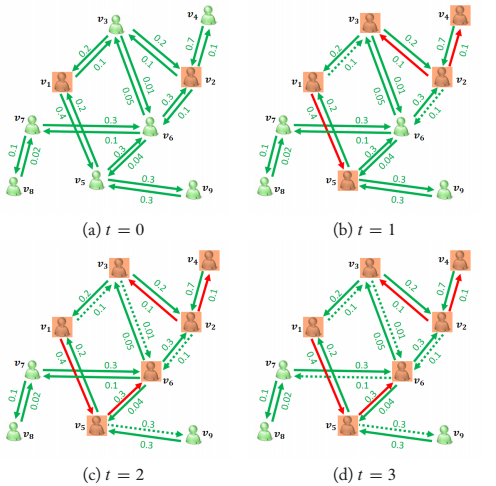
\includegraphics [scale=1]{picture/Hinh2_1}
				\end{center}
				\caption{Một số ví dụ quá trình lan truyền thông tin trên mô hình IC}
				\label{refhinh2_1}
			\end{figure}
		\end{center}
	Tại thời điểm bắt đầu t=0, hai đỉnh v$_{1}$, v$_{2}$ ở trạng thái {\itshape kích hoạt}. Ở thời điểm t = 1, v$_{1}$ kích hoạt thành công v$_{5}$ nhưng thất bại với v$_{3}$, trong khi đó v$_{2}$ kích hoạt thành công v$_{3}$ và v$_{4}$ nhưng thất bại với v$_{6}$. Tại thời điểm t = 2, v$_{3}$ kích hoạt thất bại v$_{6}$ trong khi v$_{5}$ kích hoạt thành công v$_{6}$ nhưng thất bại với v$_{9}$. Ở bước t = 3, v$_{6}$ kích hoạt thất bại v$_{7}$, đến đây quá trình lan truyền thông tin kết thúc do không có đỉnh nào được kích hoạt thêm.
	
	Mô hình IC phù hợp cho quá trình lan truyền thông tin, đó là các môi trường mà việc tiếp xúc với một nguồn là đủ để một cá nhân được kích hoạt.
	
	\subsection{Mô hình ngưỡng tuyến tính}
	Mô hình ngưỡng tuyến tính (Linear Threshold – LT) là mô hình khuếch tán ngẫu nhiên được đề xuất bởi Kempe \cite{kemple1}. Trong mô hình LT, mỗi cạnh (u,v) $\in$ [0,1] biểu diễn mức độ ảnh hưởng của đỉnh u đến đỉnh v. Nếu (u,v) $\notin$ E thì w(u,v)=0. Các trọng số này được chuẩn hóa sao cho với mỗi đỉnh v, tổng trọng số tất cả các cạnh đi đến đỉnh v lớn nhất bằng 1, tức là: $\sum_{u\in N_{in}(v)}w(u,v) \leq 1.$ 
	
	Tùy vào đặc tính của từng người dùng tương ứng, mỗi đỉnh v $\in$ V có một giá trị $\theta$$_{v}$ $\in$ [0,1], biểu diễn ngưỡng đỉnh v bị ảnh hưởng bởi các đỉnh kích hoạt hàng xóm. Quá trình lan truyền thông tin trên mô hình LT diễn ra theo bước thời gian rời rạc, tạo ra tập các đỉnh kích hoạt theo quy tắc sau:
	\begin {itemize}
		\item Tại thời điểm t = 0, tập đỉnh ở trạng thái kích hoạt chính là tập nguồn phát thông tin sai lệch S$_{0}$.
	
		\item Tại thời điểm t $\geq$ 1, đầu tiên ta gán S$_{t}$ bằng S$_{t-1}$. Sau đó với mỗi đỉnh chưa được kích hoạt v $\in$ V \ S$_{t-1}$, nếu tổng ảnh hưởng từ những đính hàng xóm kích hoạt tới v vượt ngưỡng $\theta$$_{0}$, tức là  $\sum_{u\in S_{t-1} \cap N_{in}(v)}w(u,v) \geq \theta_{v}$ thì đỉnh v được kích hoạt, ta thêm v vào tập S$_{t}$.
	
		\item Nếu tại thời điểm t, không có nút nào được kích hoạt thêm nữa, nghĩa là S$_{t}$ = S$_{t-1}$, tập các nút kích hoạt sẽ không còn thay đổi nữa, và quá trình truyền tin kết thúc với tập các nút bị kích hoạt cuối cùng là S$_{t}$.
	\end {itemize}
	Sự ngẫu nhiên trong việc lựa chọn ngưỡng $\theta$$_{0}$ từ 0 đến 1 phản ánh sự thiếu thông tin về ngưỡng nội bộ của mỗi cá nhân. Điều này phản ánh khá đúng với thực tế xã hội, bởi vì sự chập nhận thông tin của mỗi người, tại những thời điểm khác nhau là khác nhau, và rất khó để nắm bắt. 
	
	Hình \ref{refhinh2_2} chỉ ra một ví dụ quá trình lan truyền thông tin trên mô hình LT. Các đỉnh màu da cam và màu xanh tương ứng biểu diễn các đỉnh ở trạng thái {\itshape kích hoạt}, và {\itshape không kích hoạt}. Các cạnh liền màu đỏ cùng đến đỉnh v biểu diễn các cạnh này đồng thời cố thử kích hoạt đỉnh v và thành công.
	
	\begin{center}
		\begin{figure}[H]
			\begin{center}
				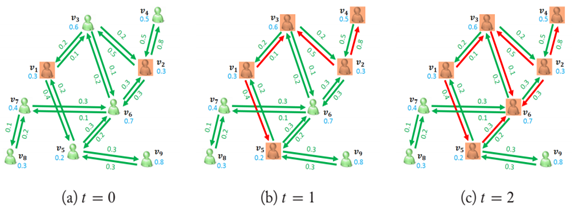
\includegraphics [scale=1]{picture/Hinh2_2}
			\end{center}
			\caption{Ví dụ quá trình lan truyền trên mô hình LT}
			\label{refhinh2_2}
		\end{figure}
	\end{center}	
	Tại thời điểm t=0, tất cả các đỉnh được khởi tạo ngẫu nhiên ngưỡng $\theta$$_{0}$ $\in$ [0,1], hai đỉnh v$_{1}$ và v$_{2}$ là các đỉnh hạt giống. Ở thời điểm t = 1, v$_{1}$ và v$_{2}$ kích hoạt thành công v$_{3}$, v$_{1}$ cũng phải cách hoạt thành công v$_{5}$ và v$_{2}$ kích hoạt thành công v$_{4}$; tuy nhiên v$_{6}$ lại không kích hoạt thành công vì tổng trọng số các cạnh đi đến v$_{6}$ là 0.3, trong khi ngưỡng kích hoạt của v$_{6}$ 0.7. Tại thười điểm t = 2, các đỉnh hàng xóm đi đến v$_{6}$ là v$_{2}$, v$_{3}$, v$_{5}$ đã được kích hoạt cho nên tổng trọng số các cạnh đi đến là 0.7 đủ để kích hoạt v$_{6}$. Tại bước t = 3, quá trình lan truyền thông tin kết thúc do không có đỉnh nào được kích hoạt thêm.

